\section{Grafana}\label{sec:Grafana}
Grafana ist eine Open-Source-Software zur plattformübergreifenden Analyse von Metriken und Daten. Als Webservice gehostet, ermöglicht Grafana die Visualisierung von Daten mithilfe von vorgefertigten Vorlagen für Tabellen und Graphen. Die Software unterstützt verschiedene Datenquellen und kann problemlos direkt mit einer relationalen Datenbanken verbunden werden. Grafana erleichtert somit die präzise Darstellung und Interpretation von Informationen durch benutzerfreundliche Visualisierungstools. \cite{GrafanaWebsite}\\
\vspace{-1cm}
\begin{center}
    \begin{figure}[h]
     \centering
     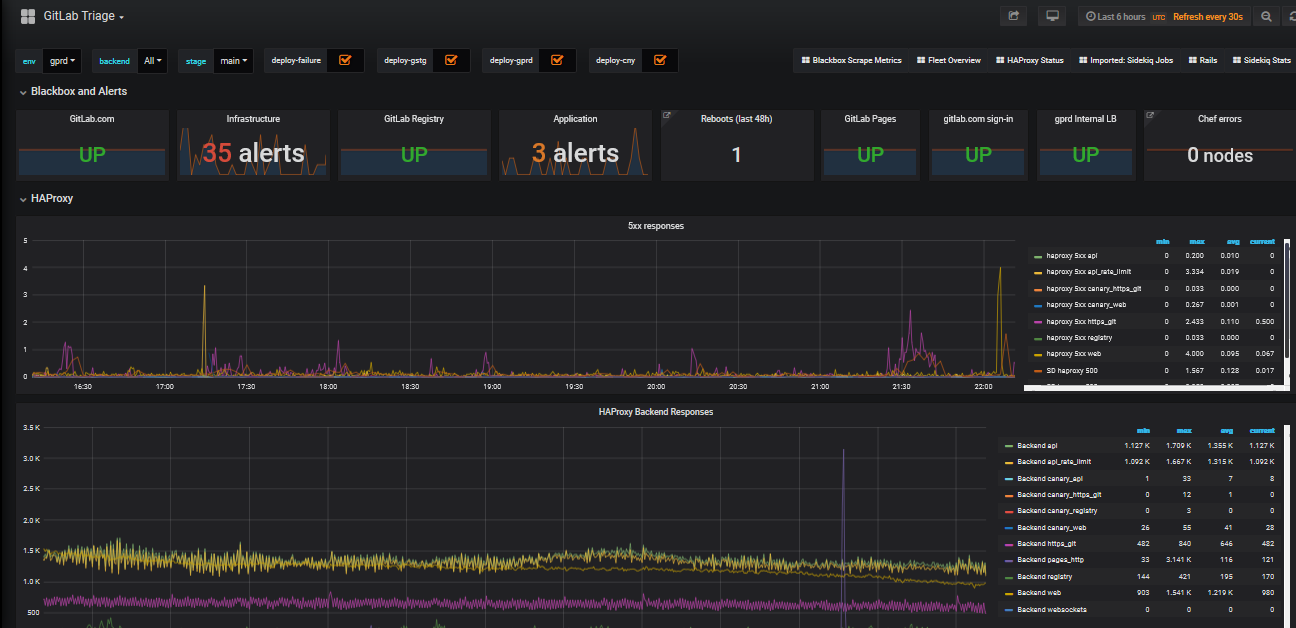
\includegraphics[width=1\textwidth]{Gitlab_Dashboard.png}
     \caption{Grafana Dashboard Beispiel \cite{GrafanaWebsite}}
     \label{fig:GRafanaDashboard}
    \end{figure}
   \end{center}
